%%%%%%%%%%%%%%%%%%%%%%%%%%%%%%%%%%%%%%%%%%%%%%%%%%%%%%%%%%%%%%%%%%%%%%%%
% Uni Duesseldorf
% Lehrstuhl fuer Datenbanken und Informationssysteme
% Vorlage fuer Bachelor-/Masterarbeiten
% Optimiert fuer den Original-Latex-Kompiler LATEX.EXE (LaTeX=>PS=>PDF)
%%%%%%%%%%%%%%%%%%%%%%%%%%%%%%%%%%%%%%%%%%%%%%%%%%%%%%%%%%%%%%%%%%%%%%%%
% Ueberarbeitung f�r pdflatex (LaTeX=>PDF)
%%%%%%%%%%%%%%%%%%%%%%%%%%%%%%%%%%%%%%%%%%%%%%%%%%%%%%%%%%%%%%%%%%%%%%%%
% Vorlage Changelog:
% 10.09.2015 (Matthias Liebeck): Nummerierung des Inhaltsverzeichnis nun r�misch, Beispiel f�r einen Anhang eingebaut, \raggedbottom %hinter sections eingefügt
%%%%%%%%%%%%%%%%%%%%%%%%%%%%%%%%%%%%%%%%%%%%%%%%%%%%%%%%%%%%%%%%%%%%%%%%
%%%% BEGINN EINSTELLUNG FUER DIE ARBEIT. UNBEDINGT ERFORDERLICH! %%%%%%%
%%%%%%%%%%%%%%%%%%%%%%%%%%%%%%%%%%%%%%%%%%%%%%%%%%%%%%%%%%%%%%%%%%%%%%%%
% Geben Sie Ihren Namen hier an:
\newcommand{\bearbeiter}{Michael Janschek}

% Geben Sie hier den Titel Ihrer Arbeit an:
\newcommand{\titel}{Klassifikation von Daten des ATLAS-Experiments}

% Geben Sie das Datum des Beginns und Ende der Bachelorarbeit ein:
\newcommand{\beginndatum}{10. Dezember 2015}
\newcommand{\abgabedatum}{10.~M�rz~2016}

% Geben Sie die Namen des Erst- und Zweitgutachters an:
\newcommand{\erstgutachter}{Prof. Dr.~Stefan Harmeling}
\newcommand{\zweitgutachter}{Prof. Dr.~Stefan Conrad}

% Falls Sie die Arbeit zweiseitig ausdrucken wollen,
% benutzen Sie die folgende Zeile mit
% \AN fuer zweiseitigen Druck
% \AUS fuer einseitigen Druck
\newcommand{\zweiseitig}{\AN}

% Falls die Arbeit in englischer Sprache verfasst 
% werden soll, dann benutzen Sie die folgende Zeile mit
% englisch fuer englische Sprache
% deutsch fuer deutsche Sprache
\newcommand{\sprache}{deutsch}

% Hier wird eingestellt, ob es sich bei der Arbeit um eine Bachelor- 
% oder Masterarbeit handelt (unpassendes auskommentieren!):
\newcommand{\arbeit}{Bachelorarbeit}
%~ \newcommand{\arbeit}{Masterarbeit}


%%%%%%%%%%%%%%%%%%%%%%%%%%%%%%%%%%%%%%%%%%%%%%%%%%%%%%%%%%%%%%%%%%%%%%%%
%%%% ENDE EINSTELLUNGEN %%%%%%%%%%%%%%%%%%%%%%%%%%%%%%%%%%%%%%%%%%%%%%%%
%%%%%%%%%%%%%%%%%%%%%%%%%%%%%%%%%%%%%%%%%%%%%%%%%%%%%%%%%%%%%%%%%%%%%%%%

% Die folgende Zeile NICHT EDITIEREN oder loeschen


%%%%%%%%%%%%%%%%%%%%%%%%%%%%%%%%%%%%%%%%%%%%%%%%%%%%%%%%%%%
% Obere Titelmakros. Editieren Sie diese Datei nur, wenn
% Sie sich ABSOLUT sicher sind, was Sie da tun!!!
% (Z.B. zum Abaendern der BA-Vorlage in eine MA-Vorlage)
% Uni Duesseldorf
% Lehrstuhl fuer Datenbanken und Informationssysteme
% Version 2.2 - 2.3.2010
%%%%%%%%%%%%%%%%%%%%%%%%%%%%%%%%%%%%%%%%%%%%%%%%%%%%%%%%%%%
\newcommand{\AN}{twoside}
\newcommand{\AUS}{}
\newcommand{\englisch}{}
%\newcommand{\deutsch}{\usepackage[german]{babel}}

%% Die folgenden auskommentierten Optionen dienen der automatischen
%% Erkennung des Latex-Kompilers und dem Setzen der davon abhängigen
%% Einstellungen. Bei Problem z.B. mit dem Einbinden von verschiedenen
%% Grafiktypen bei Verwendung von PdfLatex oder Latex, einfach die
%% verschiedenen \usepackage(s) ausprobieren. (Mit diesen Einstellungen
%% funktionierte diese Vorlage bei der Verwenundg von latex.exe als
%% Kompiler bei den meisten Studierenden.)

%\newif\ifpdf \ifx\pdfoutput\undefined
%\pdffalse % we are not running pdflatex
%\else
%\pdfoutput=1 % we are running pdflatex
%\pdfcompresslevel=9 % compression level for text and image;
%\pdftrue \fi



\documentclass[11pt,a4paper, \zweiseitig]{article}

%%%%%%%%%%%%%%%%%%%%%%%%%%%%%%%%%%%%%%%%%%%%%%%%%%%%%%%%%%%%%%%%%%%%%%%%%%%%%%%%
%%%%%%%%%%%%%%%%%%%%%%%%%%%%%%%%%%%%%%%%%%%%%%%%%%%%%%%%%%%%%%%%%%%%%%%%%%%%%%%%
%%%%%%%%%%%%%%%%%%%%%%%%%%%%%%%%%%%%%%%%%%%%%%%%%%%%%%%%%%%%%%%%%%%%%%%%%%%%%%%%
    
    \usepackage{graphicx} % Used to insert images
    \usepackage{adjustbox} % Used to constrain images to a maximum size 
    \usepackage{color} % Allow colors to be defined
    \usepackage{enumerate} % Needed for markdown enumerations to work
   %\usepackage{geometry} % Used to adjust the document margins
    \usepackage{amsmath} % Equations
    \usepackage{amssymb} % Equations
    \usepackage{eurosym} % defines \euro
    \usepackage[mathletters]{ucs} % Extended unicode (utf-8) support
    \usepackage[utf8x]{inputenc} % Allow utf-8 characters in the tex document
    \usepackage{fancyvrb} % verbatim replacement that allows latex
    \usepackage{grffile} % extends the file name processing of package graphics 
                         % to support a larger range 
    % The hyperref package gives us a pdf with properly built
    % internal navigation ('pdf bookmarks' for the table of contents,
    % internal cross-reference links, web links for URLs, etc.)
    \usepackage{hyperref}
    \usepackage{longtable} % longtable support required by pandoc >1.10
    \usepackage{booktabs}  % table support for pandoc > 1.12.2
    

    
    
    
%%%%%%%%%%%%%%%%%%%%%%%%%%%%%%%%%%%%%%%%%%%%%%%%%%%%%%%%%%%%%%%%%%%%%%%%%%%%%%%%
%%%%%%%%%%%%%%%%%%%%%%%%%%%%%%%%%%%%%%%%%%%%%%%%%%%%%%%%%%%%%%%%%%%%%%%%%%%%%%%%
%%%%%%%%%%%%%%%%%%%%%%%%%%%%%%%%%%%%%%%%%%%%%%%%%%%%%%%%%%%%%%%%%%%%%%%%%%%%%%%%



\usepackage[inner=4cm,outer=2cm]{geometry}
\usepackage{ifthen}
\ifthenelse{\equal{\sprache}{deutsch}}{\usepackage[ngerman]{babel}}{}


%%%%%%%%%%%%%%%%%%%%%%%%%%%%%%%%%%%%%%%%%%%%%%%%%%%%%%%%%%%%%%%%%%%%%%%%%%%%%%%%
\usepackage{color,fancyhdr}
\fancyhf{}
\pagestyle{fancy}
\definecolor{bleudefrance}{rgb}{0.0745, 0.4431, 0.7843} %HHU-Blau
\renewcommand{\headrule}
	{{\color{bleudefrance}%
		\hrule height 2pt
			width\headwidth
		\vspace{1pt}%
		\hrule height 1pt
			width\headwidth
		\vspace{-4pt}
	}
	{\renewcommand{\headrulewidth}{15cm} % remove lines as well
	}}
\renewcommand{\sectionmark}[1]{ \markboth{#1}{} }

\ifthenelse{\equal{\zweiseitig}{twoside}}
	{\fancyhead[LE]{\thepage \hskip6mm \textit{\nouppercase{\leftmark}}}}
	{\fancyhead[LO]{\textit{\nouppercase{\leftmark}}}}
\fancyhead[RO]{\textit{\nouppercase{\rightmark} \hskip6mm \thepage}}

%%%%%%%%%%%%%%%%%%%%%%%%%%%%%%%%%%%%%%%%%%%%%%%%%%%%%%%%%%%%%%%%%%%%%%%%%%%%%%%%



%\usepackage[iso]{umlaute}
\usepackage[utf8x]{inputenc}
\usepackage{palatino} % palatino Schriftart
%\usepackage{makeidx} % um ein Index zu erstellen
\usepackage[nottoc]{tocbibind}
\usepackage[T1]{fontenc} %fuer richtige Trennung bei Umlauten
\usepackage{fancybox} % fuer die Rahmen
\usepackage{shortvrb}


\usepackage{a4wide} % ganze A4 Weite verwenden

%\ifpdf
%\usepackage[pdftex,xdvi]{graphicx}
%\usepackage{thumbpdf} %thumbs fuer Pdf
%\usepackage[pdfstartview=FitV]{hyperref} %anklickbares Inhaltsverzeichnis
%\else
%\usepackage[dvips,xdvi]{graphicx}
\usepackage{graphicx}
\usepackage{hyperref} %anklickbares Inhaltsverzeichnis
%\fi

%%%%%%%%%%%%%%%%%%%%%%% Massangaben fuer die Arbeit %%%%%%%%%%%%%%%

\setlength{\textwidth}{15cm}

\setlength{\oddsidemargin}{40mm}
\setlength{\evensidemargin}{20mm}

\addtolength{\oddsidemargin}{-1in}
\addtolength{\evensidemargin}{-1in}

%\makeindex

\begin{document}

%\setcounter{secnumdepth}{4} %Nummerieren bis in die 4. Ebene
%\setcounter{tocdepth}{4} %Inhaltsverzeichnis bis zur 4. Ebene

%\pagestyle{headings}
%\pagestyle{fancy}

%%%%%%%%%%%%%%%%%%%%%%%%%%%%%%%%%%%%%%%%%%%%%%%%%%%%%%%%%%%%%%%%%%%%%%%%%%%%%%%%
\setlength{\headheight}{15pt}


%%%%%%%%%%%%%%%%%%%%%%%%%%%%%%%%%%%%%%%%%%%%%%%%%%%%%%%%%%%%%%%%%%%%%%%%%%%%%%%%


\sloppy % LaTeX ist dann nicht so streng mit der Silbentrennung
%~ \MakeShortVerb{\§}

\parindent0mm
\parskip0.5em


{
\textwidth170mm 
\oddsidemargin30mm 
\evensidemargin30mm 
\addtolength{\oddsidemargin}{-1in}
\addtolength{\evensidemargin}{-1in}

\parskip0pt plus2pt

% Die Raender muessen eventuell fuer jeden Drucker individuell eingestellt
% werden. Dazu sind die Werte fuer die Abstaende `\oben' und `\links' zu
% aendern, die von mir auf jeweils 0mm eingestellt wurden.

%\newlength{\links} \setlength{\links}{10mm}  % hier abzuaendern
%\addtolength{\oddsidemargin}{\links}
%\addtolength{\evensidemargin}{\links}

\begin{titlepage}
\vspace*{-1.5cm}
  \raisebox{17mm}{
    \begin{minipage}[t]{70mm}
      \begin{center}
        %\selectlanguage{german}
        {\Large INSTITUT FÜR INFORMATIK\\}
        {\normalsize
          Computer Vision, Computer Graphics and Pattern Recognition\\
        }
        \vspace{3mm}
        {\small Universitätsstr. 1 \hspace{5ex} D--40225 Düsseldorf\\}
     \end{center}
    \end{minipage}
  }
  \hfill
  
\includegraphics[width=130pt]{bilder/HHU_Logo}
  \vspace{14em}

% Titel
  \begin{center}
      	\baselineskip=55pt
    	\textbf{\huge \titel}
  	 	\baselineskip=0 pt
   \end{center}

  %\vspace{7em}

\vfill

% Autor
  \begin{center}
    \textbf{\Large
      \bearbeiter
    }
  \end{center}

  \vspace{35mm}
 
% Prüfungsordnungs-Angaben
  \begin{center}
    %\selectlanguage{german}
    
%%%%%%%%%%%%%%%%%%%%%%%%%%%%%%%%%%%%%%%%%%%%%%%%%%%%%%%%%%%%%%%%%%%%%%%%%
% Ja, richtig, hier kann die BA-Vorlage zur MA-Vorlage gemacht werden...
% (nicht mehr nötig!)
%%%%%%%%%%%%%%%%%%%%%%%%%%%%%%%%%%%%%%%%%%%%%%%%%%%%%%%%%%%%%%%%%%%%%%%%%
    {\Large \arbeit}

    \vspace{2em}

    \begin{tabular}[t]{ll}
      Beginn der Arbeit:& \beginndatum \\
      Abgabe der Arbeit:& \abgabedatum \\
      Gutachter:         & \erstgutachter \\
                         & \zweitgutachter \\
    \end{tabular}
  \end{center}

\end{titlepage}

}

%%%%%%%%%%%%%%%%%%%%%%%%%%%%%%%%%%%%%%%%%%%%%%%%%%%%%%%%%%%%%%%%%%%%%
\clearpage
\begin{titlepage}
  ~                % eine leere Seite hinter dem Deckblatt
\end{titlepage}
%%%%%%%%%%%%%%%%%%%%%%%%%%%%%%%%%%%%%%%%%%%%%%%%%%%%%%%%%%%%%%%%%%%%%
\clearpage
\begin{titlepage}
\vspace*{\fill}

\section*{Erklärung}

%%%%%%%%%%%%%%%%%%%%%%%%%%%%%%%%%%%%%%%%%%%%%%%%%%%%%%%%%%%
% Und hier ebenfalls ggf. BA durch MA ersetzen...
% (Auch nicht mehr nötig!)
%%%%%%%%%%%%%%%%%%%%%%%%%%%%%%%%%%%%%%%%%%%%%%%%%%%%%%%%%%%

Hiermit versichere ich, dass ich diese \arbeit~
selbstständig verfasst habe. Ich habe dazu keine anderen als die
angegebenen Quellen und Hilfsmittel verwendet.

\vspace{25 mm}

\begin{tabular}{lc}
Düsseldorf, den \abgabedatum \hspace*{2cm} & \underline{\hspace{6cm}}\\
& \bearbeiter
\end{tabular}

\vspace*{\fill}
\end{titlepage}

%%%%%%%%%%%%%%%%%%%%%%%%%%%%%%%%%%%%%%%%%%%%%%%%%%%%%%%%%%%%%%%%%%%%%
% Leerseite bei zweiseitigem Druck
%%%%%%%%%%%%%%%%%%%%%%%%%%%%%%%%%%%%%%%%%%%%%%%%%%%%%%%%%%%%%%%%%%%%%

\ifthenelse{\equal{\zweiseitig}{twoside}}{\clearpage\begin{titlepage}
~\end{titlepage}}{}

%%%%%%%%%%%%%%%%%%%%%%%%%%%%%%%%%%%%%%%%%%%%%%%%%%%%%%%%%%%%%%%%%%%%%
\clearpage
\begin{titlepage}

\begin{titlepage}
\vspace*{\fill}

%%% Die folgende Zeile nicht ändern!
\section*{\ifthenelse{\equal{\sprache}{deutsch}}{Zusammenfassung}{Abstract}}
%%% Zusammenfassung:
The Bachelor-Thesis presents the task of event selection for data analysis performed by the ATLAS experiment at CERN. The right solution of this classification problem is a key to successfully claim a discovery in particle physics, like the Higgs Boson discovery in 2012.\\
The Higgs Boson Machine Learning Challenge, hosted on Kaggle, serves as an example for this task and is further investigated in this work. Few strategies to solve are presented, the Gradient Boosting package XGBoost stood out with good prediction while having excellent runtime. Though it did not provide the winning submission it was acknowledged by the competition hosts with a special jury award.
As event selection is part of a budgeted data analysis system in ATLAS, runtime is an important factor for algorithms to be used in actual CERN applications. It is concluded that XGBoost has a good chance in replacing common tools in particle physics.

While there have been original tools created for testing and analysing several approaches to solve the task, no original classification algorithms have been designed or programmed in this work. The focus is set primarily on the analysis of existing classifiers provided by existing packages, like Logistic Regression Classification of scikit learn. 

\vspace{25 mm}

\textbf{Keywords:} Higgs  boson, Kaggle, Machine learning, Classification, Data science, scikit learn

\vspace*{\fill}
\end{titlepage}
\ifthenelse{\equal{\zweiseitig}{twoside}}{\clearpage\begin{titlepage}
~\end{titlepage}}{}


%%%%%%%%%%%%%%%%%%%%%%%%%%%%%%%%%%%%%%%%%%%%%%%%
% Untere Titelmakros. Editieren Sie diese Datei nur, wenn Sie sich
% ABSOLUT sicher sind, was Sie da tun!!!
%%%%%%%%%%%%%%%%%%%%%%%%%%%%%%%%%%%%%%%%%%%%%%%
\vspace*{\fill}
\end{titlepage}

%%%%%%%%%%%%%%%%%%%%%%%%%%%%%%%%%%%%%%%%%%%%%%%%%%%%%%%%%%%%%%%%%%%%%
% Leerseite bei zweiseitigem Druck
%%%%%%%%%%%%%%%%%%%%%%%%%%%%%%%%%%%%%%%%%%%%%%%%%%%%%%%%%%%%%%%%%%%%%
\ifthenelse{\equal{\zweiseitig}{twoside}}
  {\clearpage\begin{titlepage}~\end{titlepage}}{}
%%%%%%%%%%%%%%%%%%%%%%%%%%%%%%%%%%%%%%%%%%%%%%%%%%%%%%%%%%%%%%%%%%%%%
\clearpage \setcounter{page}{1}
\pagenumbering{roman}
\setcounter{tocdepth}{2}
\tableofcontents

%\enlargethispage{\baselineskip}
\clearpage

%%%%%%%%%%%%%%%%%%%%%%%%%%%%%%%%%%%%%%%%%%%%%%%%%%%%%%%%%%%%%%%%%%%%%
% Leere Seite, falls Inhaltsverzeichnis mit ungerader Seitenzahl und 
% doppelseitiger Druck
%%%%%%%%%%%%%%%%%%%%%%%%%%%%%%%%%%%%%%%%%%%%%%%%%%%%%%%%%%%%%%%%%%%%%
\ifthenelse{ \( \equal{\zweiseitig}{twoside} \and \not \isodd{\value{page}} \)}
	{\pagebreak \thispagestyle{empty} \cleardoublepage}{\clearpage}



\pagenumbering{arabic}
\setcounter{page}{1}

%%%%%%%%%%%%%%%%%%%%%%%%%%%%%%%%%%%%%%%%%%%%%%%%%%%%%%%%%%%%%%%%%%%%%%%%
%%%% BEGINN TEXTTEIL %%%%%%%%%%%%%%%%%%%%%%%%%%%%%%%%%%%%%%%%%%%%%%%%%%%
%%%%%%%%%%%%%%%%%%%%%%%%%%%%%%%%%%%%%%%%%%%%%%%%%%%%%%%%%%%%%%%%%%%%%%%%

%%%%%%%%%%%%%%%%%%%%%%%%%%%%%%%%%%%%%%%%%%%%%%%%%%%%%%%%%%%%%%%%%%%%%%%%
% Text entweder direkt hier hinein schreiben oder, im Sinne der
% besseren Uebersichtlich- und Bearbeitbarkeit mittels \input die
% einzelnen Textteile hier einbinden.
%%%%%%%%%%%%%%%%%%%%%%%%%%%%%%%%%%%%%%%%%%%%%%%%%%%%%%%%%%%%%%%%%%%%%%%%

\section{Einleitung}\raggedbottom 

\subsection{Motivation und Zielsetzung} 
%Gallia est omnis divisa in partes tres,
%quarum unam
%incolunt Belgae, aliam Aquitani, tertiam qui ipsorum lingua
%Celtae, nostra Galli appellantur. Hi omnes lingua, institutis,
%legibus inter se differunt. Gallos ab Aquitanis Garumna flumen, a
%Belgis Matrona et Sequana dividit. Horum omnium fortissimi sunt
%Belgae, propterea quod a cultu atque humanitate provinciae
%longissime absunt, minimeque ad eos mercatores saepe commeant
%atque ea quae ad effeminandos animos pertinent important,
%proximique sunt Germanis, qui trans Rhenum incolunt, quibuscum
%continenter bellum gerunt. Qua de causa Helvetii quoque reliquos
%Gallos virtute praecedunt, quod fere cotidianis proeliis cum
%Germanis contendunt, cum aut suis finibus eos prohibent aut ipsi
%in eorum finibus bellum gerunt. Eorum una, pars, quam Gallos
%obtinere dictum est, initium capit a flumine Rhodano, continetur
%Garumna flumine, Oceano, finibus Belgarum, attingit etiam ab
%Sequanis et Helvetiis flumen Rhenum, vergit ad septentriones.
%Belgae ab extremis Galliae finibus oriuntur, pertinent ad
%inferiorem partem fluminis Rheni, spectant in septentrionem et
%orientem solem. Aquitania a Garumna flumine ad Pyrenaeos montes et
%eam partem Oceani quae est ad Hispaniam pertinet; spectat inter
%occasum solis et septentriones.


\subsection{Vorgehensweise}
%Apud Helvetios longe nobilissimus fuit et
%ditissimus
%Orgetorix. Is M. Messala, [et P.] M. Pisone consulibus regni
%cupiditate inductus coniurationem nobilitatis fecit et civitati
%persuasit ut de finibus suis cum omnibus copiis exirent: perfacile
%esse, cum virtute omnibus praestarent, totius Galliae imperio
%potiri. Id hoc facilius iis persuasit, quod undique loci natura
%Helvetii continentur: una ex parte flumine Rheno latissimo atque
%altissimo, qui agrum Helvetium a Germanis dividit; altera ex parte
%monte Iura altissimo, qui est inter Sequanos et Helvetios; tertia
%lacu Lemanno et flumine Rhodano, qui provinciam nostram ab
%Helvetiis dividit. His rebus fiebat ut et minus late vagarentur et
%minus facile finitimis bellum inferre possent; qua ex parte
%homines bellandi cupidi magno dolore adficiebantur. Pro
%multitudine autem hominum et pro gloria belli atque fortitudinis
%angustos se fines habere arbitrabantur, qui in longitudinem milia
%passuum CCXL, in latitudinem CLXXX patebant.
%
%His rebus adducti et auctoritate Orgetorigis permoti constituerunt
%ea quae ad proficiscendum pertinerent comparare, iumentorum et
%carrorum quam maximum numerum coemere, sementes quam maximas
%facere, ut in itinere copia frumenti suppeteret, cum proximis
%civitatibus pacem et amicitiam confirmare. Ad eas res conficiendas
%biennium sibi satis esse duxerunt; in tertium annum profectionem
%lege confirmant. Ad eas res conficiendas Orgetorix deligitur. Is
%sibi legationem ad civitates suscipit. In eo itinere persuadet
%Castico, Catamantaloedis filio, Sequano, cuius pater regnum in
%Sequanis multos annos obtinuerat et a senatu populi Romani amicus
%appellatus erat, ut regnum in civitate sua occuparet, quod pater
%ante habuerit; itemque Dumnorigi Haeduo, fratri Diviciaci, qui eo
%tempore principatum in civitate obtinebat ac maxime plebi acceptus
%erat, ut idem conaretur persuadet eique filiam suam in matrimonium
%dat. Perfacile factu esse illis probat conata perficere, propterea
%quod ipse suae civitatis imperium obtenturus esset: non esse
%dubium quin totius Galliae plurimum Helvetii possent; se suis
%copiis suoque exercitu illis regna conciliaturum confirmat. Hac
%oratione adducti inter se fidem et ius iurandum dant et regno
%occupato per tres potentissimos ac firmissimos populos totius
%Galliae sese potiri posse sperant. (siehe \cite{Con97},
%\cite{PeHe97} und Abbildung \ref{fig_Gallien})
%
%
%\begin{figure}[htb]
%\begin{center}
%  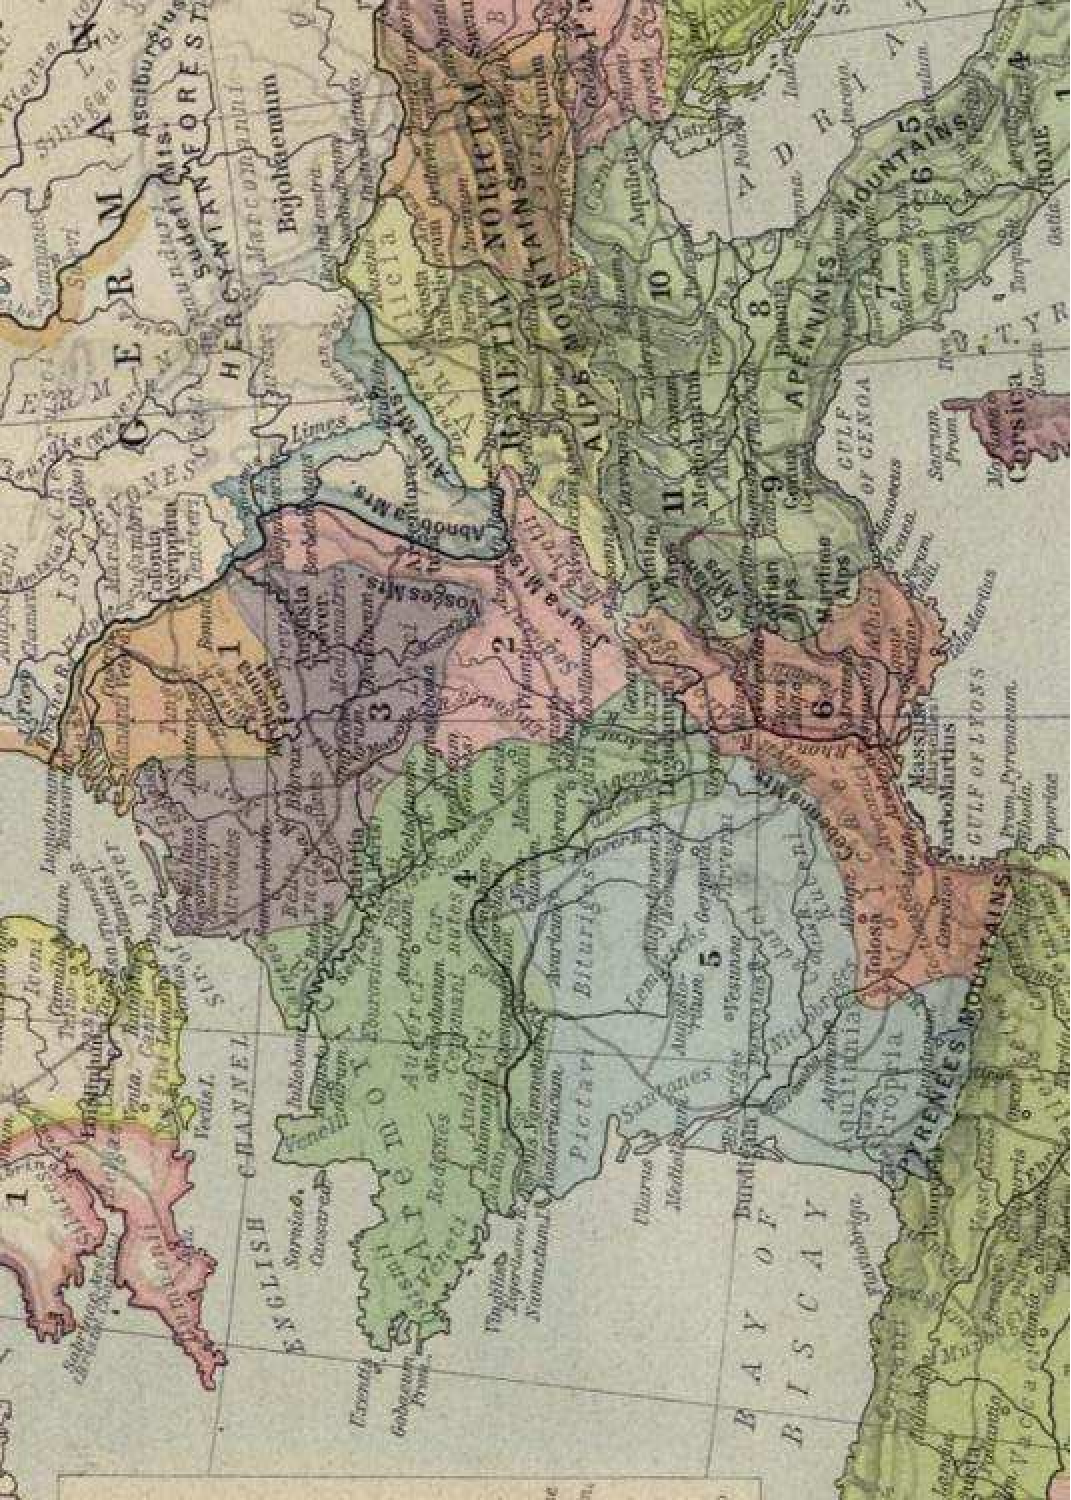
\includegraphics[width=175pt, angle=270]{bilder/Galia}
%  \caption{Gallien zur Zeit Caesars}\label{fig_Gallien}
%\end{center}
%\end{figure}
%
%
%\begin{table}[htb]
%\begin{center}
%\begin{tabular}{|l|l|l|}
%\hline
%Jahr &  Erster Consul & Zweiter Consul\\
%\hline \hline
%1 & C. Caesar         & L. Aemilius Paullus\\
%2 & P. Vinicius       & P. Alfenus Varus\\
%3 & L. Aelius Lamia   & M. Servilius\\
%4 & Sex. Aelius Catus &  C. Sentius Saturninus\\
%5 & L. Valerius Messalla& Cn. Cornelius Cinna \\
%suff. & C. Vibius Postumus &  C. Ateius Capito\\
%6 & M. Aemilius Lepidus & L. Arruntius\\
%\hline
%\end{tabular}
% \caption{Römische Konsulen}\label{tab_Konsulen}
%\end{center}
%\end{table}


\pagebreak

\section{Definitionen und Grundlagen}\raggedbottom
\subsection{Das formale Problem}
\subsection{Evaluation}
\subsection{Die Daten}

%Pharnace superato, Africa recepta, qui ex his proeliis cum
%adulescente Cn. Pompeio profugissent, cum . . . et ulterioris
%Hispaniae potitus esset, dum Caesar muneribus dandis in Italia
%detinetur, . . . quo facilius praesidia contra compararet,
%Pompeius in fidem uniuscuiusque civitatis confugere coepit. Ita
%partim precibus partim vi bene magna comparata manu provinciam
%vastare. Quibus in rebus non nullae civitates sua sponte auxilia
%mittebant, item non nullae portas contra cludebant. Ex quibus si
%qua oppida vi ceperat, cum aliquis ex ea civitate optime de Cn.
%Pompeio meritus civis esset, propter pecuniae magnitudinem alia
%qua ei inferebatur causa, ut eo de medio sublato ex eius pecunia
%latronum largitio fieret. Ita pacis commoda hoste +hortato+
%maiores augebantur copiae. +Hoc crebris nuntiis in Italiam missis
%civitates contrariae Pompeio+ auxilia sibi depostulabant.
%
%C. Caesar dictator tertio, designatus dictator quarto multis
%+iterante diebus coniectis+ cum celeri festinatione ad bellum
%conficiendum in Hispaniam cum venisset, legatique Cordubenses, qui
%a Cn. Pompelo discessissent, Caesari obviam venissent, a quibus
%nuntiabatur nocturno tempore oppidum Cordubam capi posse, quod nec
%opinantibus adversariis eius provinciae potitus esset, simulque
%quod tabellariis, qui a Cn. Pompeio dispositi omnibus locis
%essent, qui certiorem Cn. Pompeium de Caesaris adventu facerent .
%. . multa praeterea veri similia proponebant. Quibus rebus
%adductus quos legatos ante exercitui praefecerat Q. Pedium et Q.
%Fabium Maximum de suo adventu facit certiores, utque sibi
%equitatus qui ex provincia fuisset praesidio esset. Ad quos
%celerius quam ipsi opinati sunt appropinquavit neque, ut ipse
%voluit, equitatum sibi praesidio habuit.
%
%Erat idem temporis Sex. Pompeius frater qui cum praesidio Cordubam
%tenebat, quod eius provinciae caput esse existimabatur; ipse autem
%Cn. Pompeius adulescens Uliam oppidum oppugnabat et fere iam
%aliquot mensibus ibi detinebatur. Quo ex oppido cognito Caesaris
%adventu legati clam praesidia Cn. Pompei Caesarem cum adissent,
%petere coeperunt uti sibi primo quoque tempore subsidium mitteret.
%Caesar - eam civitatem omni tempore optime de populo Romano
%meritam esse - celeriter sex cohortis secunda vigilia iubet
%proficisci, pari equites numero. Quibus praefecit hominem eius
%provinciae notum et non parum scientem, L. Vibiurn Paciaecum. Qui
%cum ad Cn. P praesidia venisset, incidit idem temporis ut
%tempestate adversa vehementique vento adflictaretur; aditusque vis
%tempestatis ita obscurabat ut vix proximum agnoscere possent.
%Cuius incommodum summam utilitatem ipsis praebebat. Ita cum ad eum
%locum venerunt, iubet binos equites conscendere, et recta per
%adversariorum praesidia ad oppidum contendunt. Mediisque eorum
%praesidiis cum essent, cum quaereretur qui essent unus ex nostris
%respondit, ut sileat verbum facere: nam id temporis conari ad
%murum accedere, ut oppidum capiant; et partim tempestate impediti
%vigiles non poterant diligentiam praestare, partim illo responso
%deterrebantur. Cum ad portam appropinquassent, signo dato ab
%oppidanis sunt reccepti, et pedites dispositi partim ibi
%remanserunt, equites clamore facto eruptionem in adversariorum
%castra fecerunt.

\pagebreak
\section{Lösungsstrategien}\raggedbottom 
\subsection{Eigene Ansätze}
\subsubsection{Logstic Regression}
\subsubsection{k-Nearest-Neighbours}
\subsection{Neural Networks}
\subsection{Regularized Greedy Forest}
\subsection{XGBoost}

%%%%%%%%%%%%%%%%%%%%%%%%%%%%%%%%%%%%%%%%%%%%%%%%%%%%%%%%%%%%%%%%%%%%%%%%
%%%% ENDE TEXTTEIL %%%%%%%%%%%%%%%%%%%%%%%%%%%%%%%%%%%%%%%%%%%%%%%%%%%%%
%%%%%%%%%%%%%%%%%%%%%%%%%%%%%%%%%%%%%%%%%%%%%%%%%%%%%%%%%%%%%%%%%%%%%%%%

\clearpage

% Entfernen Sie das Kommentar aus der nachfolgenden Zeile, falls Sie einen Anhang in der Arbeit verwenden wollen. Beachten Sie, dass Sie sich im Verlauf der Arbeit mit \ref{...} (z.B. \ref{anhang:zusatz1}) auf den Anhang beziehen.
%\newpage
\appendix
\section{Anhang}

\subsection*{Zusatzteil 1} \label{anhang:zusatz1}

Dies ist ein Anhang.

\clearpage

\bibliography{references}
\bibliographystyle{alphadin}
%\vspace*{\fill}

\clearpage

\listoffigures

\listoftables

%\pagebreak

%\printindex
\end{document}
